%%%%%%%%%%%%%%%%%%%%%%%%%%%%%%%%%%%%%%%%%%%%%%%%%%%%%%%%%%%%%%%%%%%%%%%%%%%%%%%%
%2345678901234567890123456789012345678901234567890123456789012345678901234567890
%        1         2         3         4         5         6         7         8
% THESIS Chapter

\chapter{Background}

\section{Current Dynamic Network Visualisation Techniques}

In 2014 an investigation was done into the state of the art of visualising the dynamic element or third dimension \cite{tsotaivg}. Whilst this report will focus on using measure visualisations as a dynamic network visualisation technique it can be useful to see how the temporal element was directly visualised at a network level.

One such dynamic visualisation technique is using 'animations' or 'movies'. SoNIA \cite{sonia} for example is a node-link animation based dynamic network visualisation tool that aims "to handle network data and visualization in ways that explicitly deal with its time-based nature and aids the user in understanding what their data really mean" \cite{taasodnv}. SoNIA can be used to save the network animation as a quicktime movie. An interesting technique used in SoNIA is the interpolation of points between changes, to create smoother transitions that are more easily followed by the human eye. SoNIA has been successfully used for modelling interaction networks, disease transmission and football passing patterns demonstrating that animations are a feasible tool for visualising changes in network structure.

A common method of visualising static networks is the use of an adjacency matrix. Matrix Cubes \cite{vdnwmc} applies this technique to dynamic networks. Matrix cubes take the adjacency matrix of each static slice of a dynamic network and stacks them next to each other in order - using time as the third dimension, creating a cube. 
%Matrixes are more readable for larger and denser graphs with nodelink found to be worse than a matrix representation for static networks composed of over 20 nodes \cite{acotrogunlambr}.

When using a series of static node-link diagrams there are two methods to visualise the changes - one after the other (time-multiplexed) or side by side (juxtaposed) \cite{vdnwmc}. 


While The Vistorian's node-link diagram is timeline based the novel approach taken in this report is measure based and visualised alongside the existing timeline based approach. Since the local measures values are calculated based on the time window set in the timeline and the global measures use it directly as an axis, the measure based approach is tightly intertwined with the timeline approach. The measures themselves and their own accompanying visualisations are used to aid user's understanding of the networks changes - complementing the  timeline approach rather than replacing it.


\subsection{Measures}
A static measure, for example degree centrality, quantifies some aspect of a static network. They can be either local - based on a single node, or global - based on the network as a whole. Density is an example of a global static measure. 

Dynamic measures on the other hand fall into two categories. In the first category are measures which only make sense in a dynamic context and could not be applied to a strictly static network. In the second, static measures are applied and calculated at each time-frame, where a time-frame is the unit of change. %more?
Dynamic measures can also be described as local or global.



\section{Technologies}
\subsection{JavaScript and D3}
\label{sec:sec24}
The Vistorian was primarily written in TypeScript and D3 \cite{d3site}. Since I'm more comfortable working directly with Javascript all code was implemented using Javascript. D3 was used for the visualisations.

\subsection{Vistorian Implementation}

\begin{center}
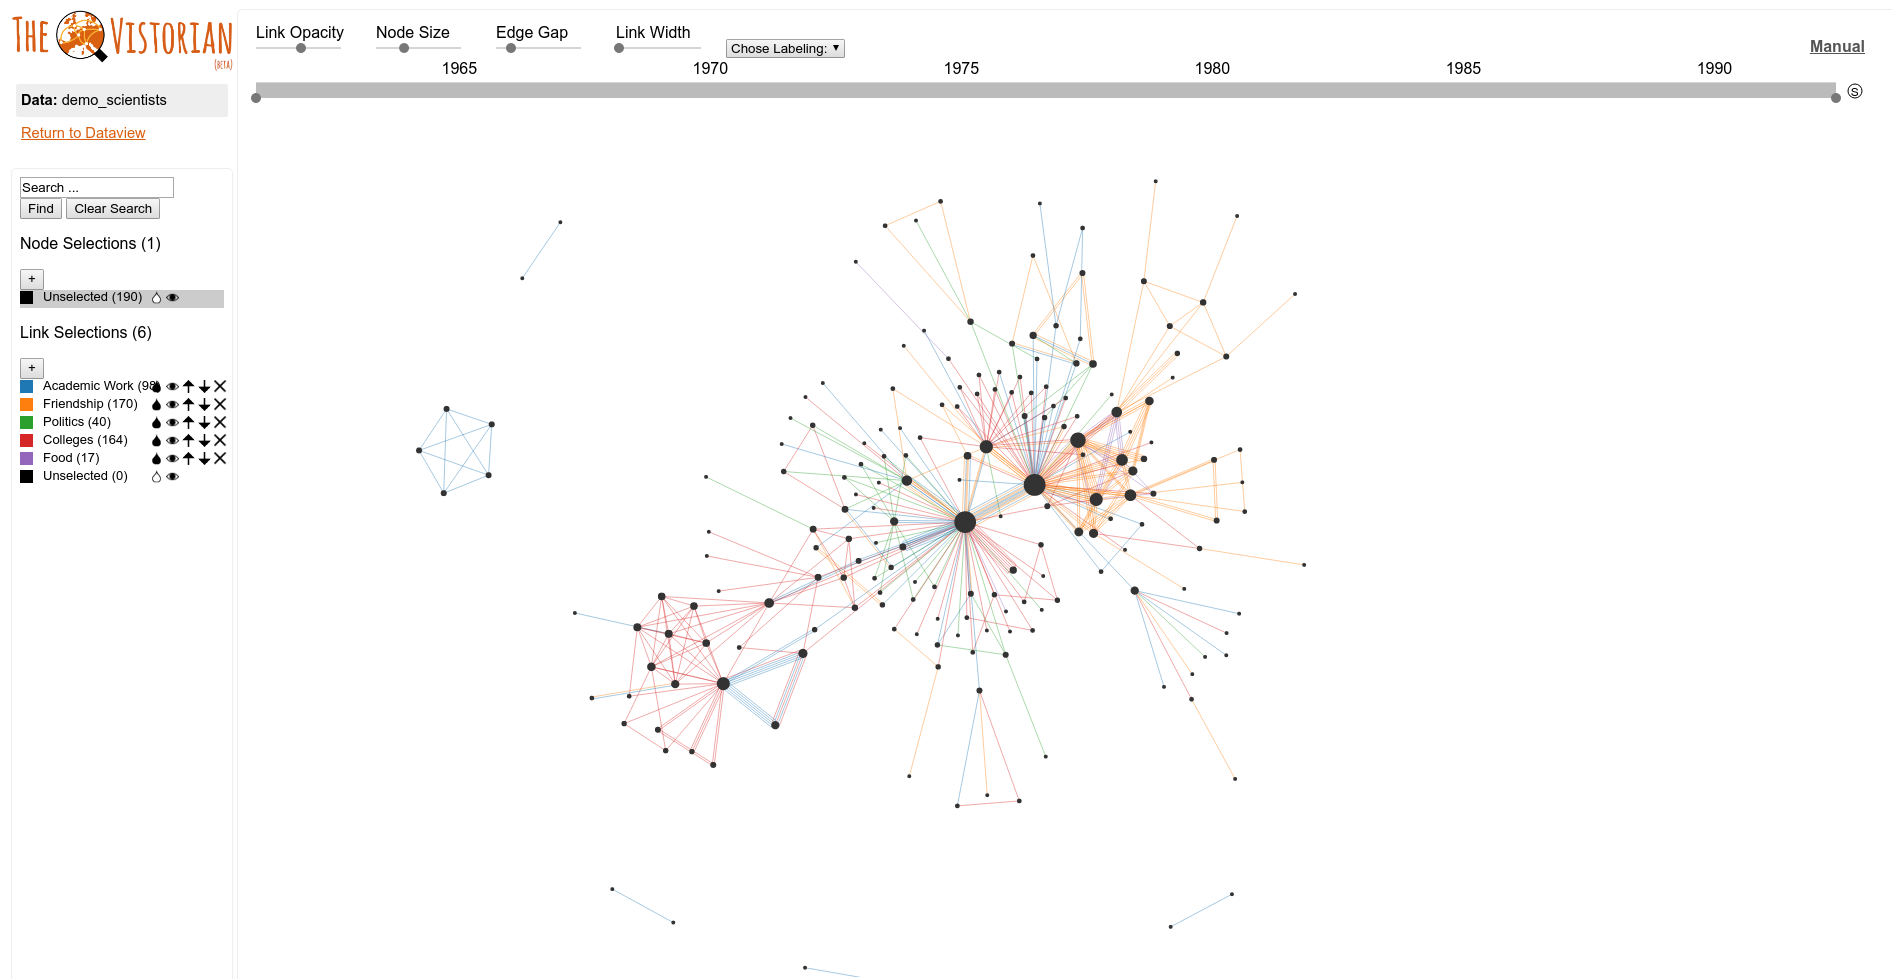
\includegraphics[trim={0 0 0 0}, width=140mm]{./Figures/vistorianOriginal.png}
\end{center}

More details are given in the visualization manual \cite{vismanual} but a summary of the key aspects is provided below.
This project will focus on the ‘Node-link’ visualisation specifically. The node-link diagram is composed of nodes as points and edges as straight lines. The positions of nodes are kept the same for all time-frames, making it easier to visualise \cite{tsotaivg} and preserving the user's mental map\cite{}. It's also simple and intuitive.
%-Node-link history and development, why I'm using this one.\newline <-?
At the top of the network page is a time-slider. Adjusting this time slider filters the links shown if they are not present in that window. A force-directed layout is used, meaning that nodes with many common neighbours are drawn close to each other and nodes with fewer connections are moved to the edges. Node size is used to indicate the node degree and line colour indicates a specific type of relation. Edges are defined as the direct links between nodes and only exist during at most one time-frame, whereas a nodepair is active if any edge is present between two nodes - meaning they can exist during multiple time-frames provided there is at least one edge linking the nodes. In The Vistorian the network is split into discrete time-frames where each time-frame represents some change happening in the network. 





